\section{Clustering and Profiling}

The process of clustering begins with the generation of a dendogram using Gower-Ward's method

\begin{figure}[H]
    \centering
    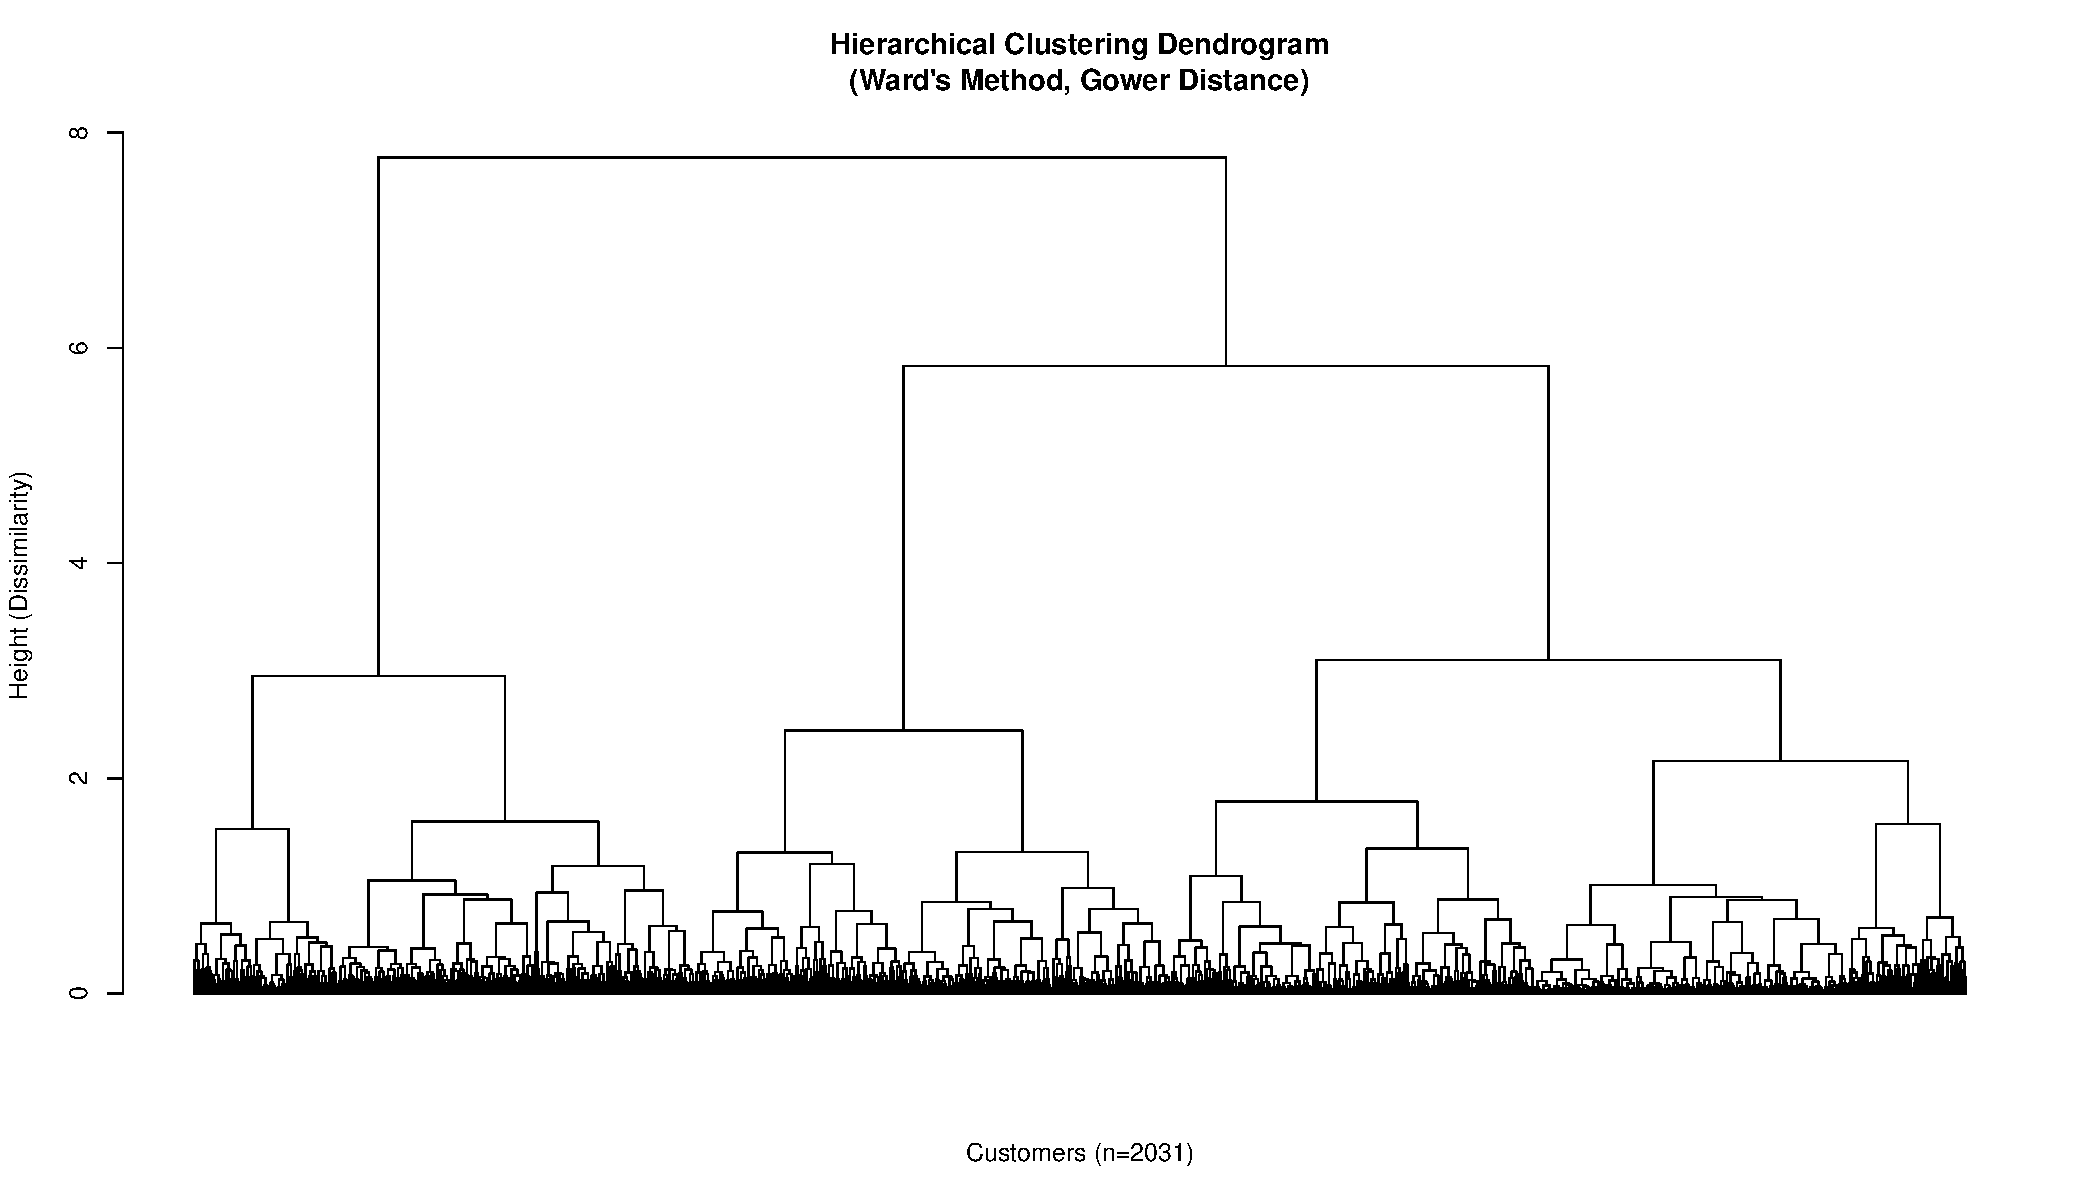
\includegraphics[width=1\linewidth]{Imatges/dendrogram_Gower_Ward.pdf}
    \caption{Dendogram}
    \label{fig:dend}
\end{figure}

Using the elbow method and silhouette analysis shown on Figure \ref{fig:optdig}, we determine that $k = 3$ is the appropiate decision to move forward

\begin{figure}[H]
    \centering
    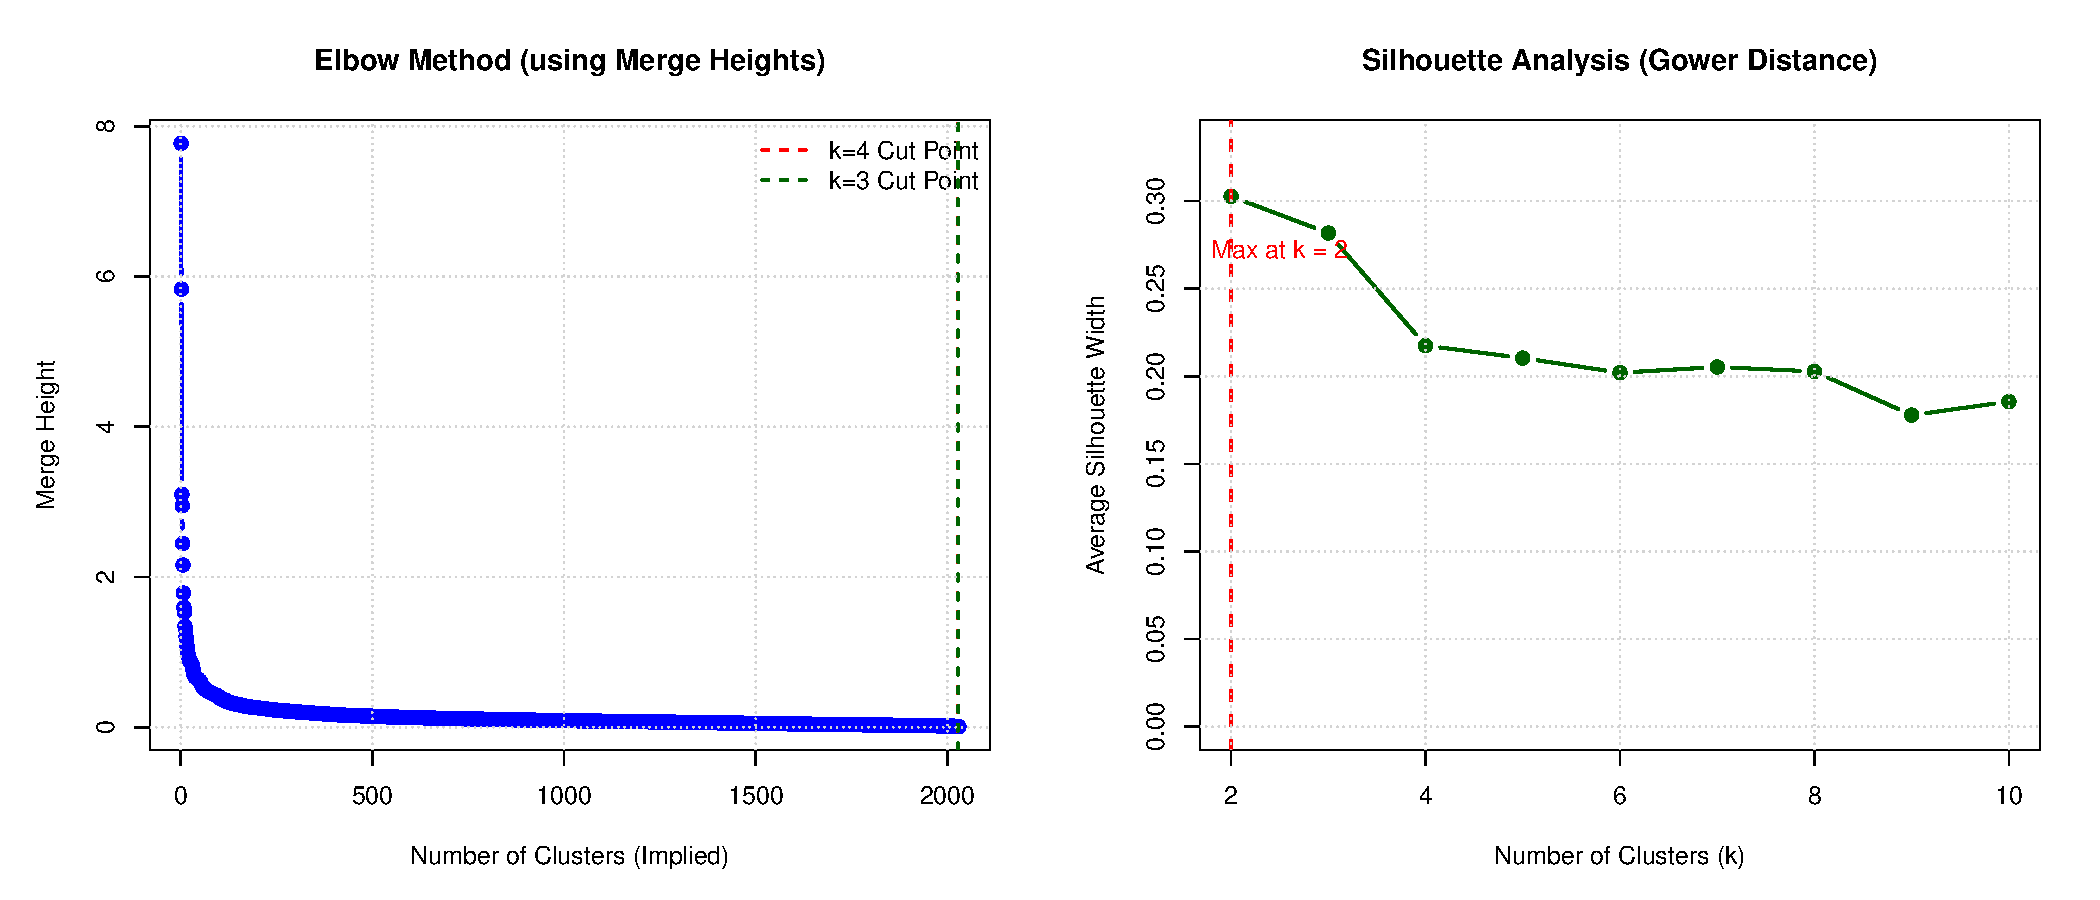
\includegraphics[width=1\linewidth]{Imatges/Clustering_OptimalK_Diagnostics_Gower.pdf}
    \caption{Clustering Optimal Diagnostics}
    \label{fig:optdig}
\end{figure}
